\documentclass[letterpaper, 10pt, conference]{ieeeconf}  % 
\IEEEoverridecommandlockouts                              % This command is only needed if 
                                                          % you want to use the \thanks command
\overrideIEEEmargins    
\usepackage{cite}

\usepackage{algorithmic}

\usepackage{textcomp}

\usepackage{comment}

%\usepackage{graphicx}      % include this line if your document contains figures
%\usepackage{natbib}        % required for bibliography
%===============================================================================
% Needed to meet printer requirements.
 \usepackage{latexsym,amssymb,amsfonts}
\usepackage[applemac]{inputenc}
\usepackage{rotating}
\usepackage{cite}
%\usepackage{graphicx}
\usepackage{epstopdf}
\usepackage{subfigure}
%\usepackage{color}
%\usepackage{xcolor}
%
%\usepackage{color}
\usepackage[dvipsnames]{xcolor}
%
\usepackage[normalem]{ulem}
\usepackage{isolatin1}
%\usepackage{caption}
%\usepackage{array,multirow,makecell}
%\usepackage{placeins}
%\usepackage{stackengine}
%\usepackage{hyperref}
\usepackage{fancybox}
\usepackage{colortbl}
\usepackage{float}
\usepackage{comment}
\usepackage{mathdots}
%\usepackage{lmodern}
%%%%%%%%%%%%%%%%%%%%%%%%%%%%%%%%%%%%%%%%%%%%%%%%%%%%%%%%%
\usepackage{dblfloatfix}
\usepackage{kantlipsum}
\usepackage{dblfloatfix}    % To enable figures at the bottom of page
\usepackage{graphicx} % [demo] option for empty figure
\usepackage{placeins}
\usepackage{marginnote}
\usepackage{url}
\usepackage{hyperref}
\usepackage{fancybox}
%\usepackage{empheq}
\usepackage[overload]{empheq}

\usepackage{bm}

%%%%%%%%%%%%%%%%%%%%%%%%%%%%%%%%%%%%%%%%%%%%%%%%%%%%%%%%%
\usepackage{tikz}
\usetikzlibrary{circuits.ee.IEC}
\usepackage[european resistor, european voltage, european current]{circuitikz}
\usetikzlibrary{arrows, shapes ,positioning}
\usetikzlibrary{decorations.markings,decorations.pathmorphing,
decorations.pathreplacing}
\usetikzlibrary{calc,patterns,shapes.geometric}
\usetikzlibrary{shapes.multipart,positioning,patterns,backgrounds}
\tikzstyle{titlebox}=[rectangle,inner sep=10pt,inner ysep=10pt,draw]%
\usetikzlibrary{arrows.meta}

%%%%%%%%%%%%%%%%%%%%%%%%%%%%%%%%%%%%%%%%%%%%%%%%%%%%%%%%%%%%%

\def\blacksquare{\hbox{\vrule width 4pt height 4pt depth 0pt}}
\def\square{\hbox{\vrule\barox{\hrule\phantom{o}\hrule}\vrule}}
\def\qed{\hfill \square}
\def\qedp{\rightline{$\blacksquare$}}
\def\EXPT{\mathop{{\rm E}}}
\def\MIN{\mathop{{\rm min}}}
\def\MAX{\mathop{{\rm max}}}
\def\LIM{\mathop{{\longrightarrow}}}
\def\UNION{\mathop{\bigcup}}
\def\INTERSECT{\mathop{\bigcap}}
\def\ARGMIN{\mathop{{\rm argmin}}}
\def\ARGMAX{\mathop{{\rm argmax}}}
\def\TOUND{\mathop{\longrightarrow}}
\def\col#1{\mathop{{\rm col}\,\left(\,#1\,\right)}}
\def\eqref#1{(\ref{#1})}
\def\rank{\mathop{{\rm rank}}}

\newcommand{\widebox}[2][0.5em]{\fbox{\hspace{#1}$\displaystyle #2$\hspace{#1}}}



\def\rank{\mathop{{\rm rank}}}

% User definition from Shengya
\def\V{\mathcal{V}} % the set of vehicle
\def\E{\mathcal{E}} % the set of edge
\def\G{\mathcal{G}} % graph
\def\A{\mathcal{A}} % adjacency matrix 
\def\W{\mathcal{W}} % weighted adjacency matrix
\def\L{\mathcal{L}} % Laplacian matrix
\def\N{\mathcal{N}} % neighbors
\def\LO{\mathcal{LO}} % the set of observer
\def\DO{\mathcal{DO}} % the set of observer
\def\diag#1{\mathop{{\rm diag}\,\left(\,#1\,\right)}}
\def\ST{\mathcal{ST}} % Self trust
\def\LT{\mathcal{LT}} % Local trust
\def\DT{\mathcal{DT}} % Distributed trust 
\def\VT{\mathcal{VT}} % Vehicle trust 
\def\AT{\mathcal{AT}} % Aggregation trust
\def\T{\mathcal{T}} % Aggregation trust
\def\O{\mathcal{O}} % opinion


% User Defined Color based on RGB
\definecolor{blue1}{RGB}{31,119,180} 
\definecolor{orange1}{RGB}{255,127,14} 
\definecolor{green1}{RGB}{44,160,44}    
\definecolor{purple1}{RGB}{148,103,189}
\definecolor{rose1}{RGB}{227, 119, 194}


%%%
\newtheorem{prb}{\it Problem}%[section]
\newtheorem{theorem}{\it Theorem}%[section]
\newtheorem{lemma}{\it Lemma}%[section]
\newtheorem{definition}{\it Definition}
\newtheorem{remark}{\it Remark}%[section]
\newtheorem{assumption}{\it Assumption}%[section]
\newtheorem{example}{\it Example}%[section]b
\newtheorem{annex}{\it Annex}%[section]b
\newtheorem{prop}{\it Proposition}%[section]b

\newtheorem{alert}{\color{red}\it Alert Remark}
\newtheorem{proof}{\it Proof}%[section]b


% 自定义色彩
\definecolor{blue1}{RGB}{31,119,180}    % 车辆/物理层
\definecolor{orange1}{RGB}{255,127,14}  % 本地观测器
\definecolor{green1}{RGB}{44,160,44}    % 信息层/通信
\definecolor{purple1}{RGB}{148,103,189} % 分布式观测器




\def\BibTeX{{\rm B\kern-.05em{\sc i\kern-.025em b}\kern-.08em
    T\kern-.1667em\lower.7ex\hbox{E}\kern-.125emX}}

\begin{document}


\title{\bf Resilience in Distributed
 Consensus based on Trust for Connected Vehicle }
\author{Q.H. Nguyen$^{1,2}$, Shengya Meng $^{1}$, H. Rafaralahy $^{1}$, M. Haddad $^{2}$, A. Zemouche $^{1}$
%
\thanks{This work was supported by SEGULA Engineering. H. Rafaralahy and A. Zemouche would like to acknowledge the ANR agency for its partial financial support under the project ArtISMo ANR-20-CE48-0015.
}
%
\thanks{$^{1}$ Universit\'e de Lorraine, CNRS, CRAN, F-57000 Metz, France~(e-mail: \protect\url{ali.zemouche@univ-lorraine.fr}).}
%
\thanks{$^{2}$ SEGULA Engineering, 19 rue d'Arras, 92000 Nanterre, France~(e-mail: \protect\url{madjid.haddad@segula.fr}).}
%
\thanks{All relevant CARLA resources have been made available in \protect\href{https://github.com/kslhuy/CACC_UIO_simulink}{GitHub}.}
}
\maketitle

\begin{abstract}

\end{abstract}

\begin{keywords}
Distributed observers, secure estimation, lyapunov stability, cyber-attack.
\end{keywords}


\begin{figure*}
\centering
    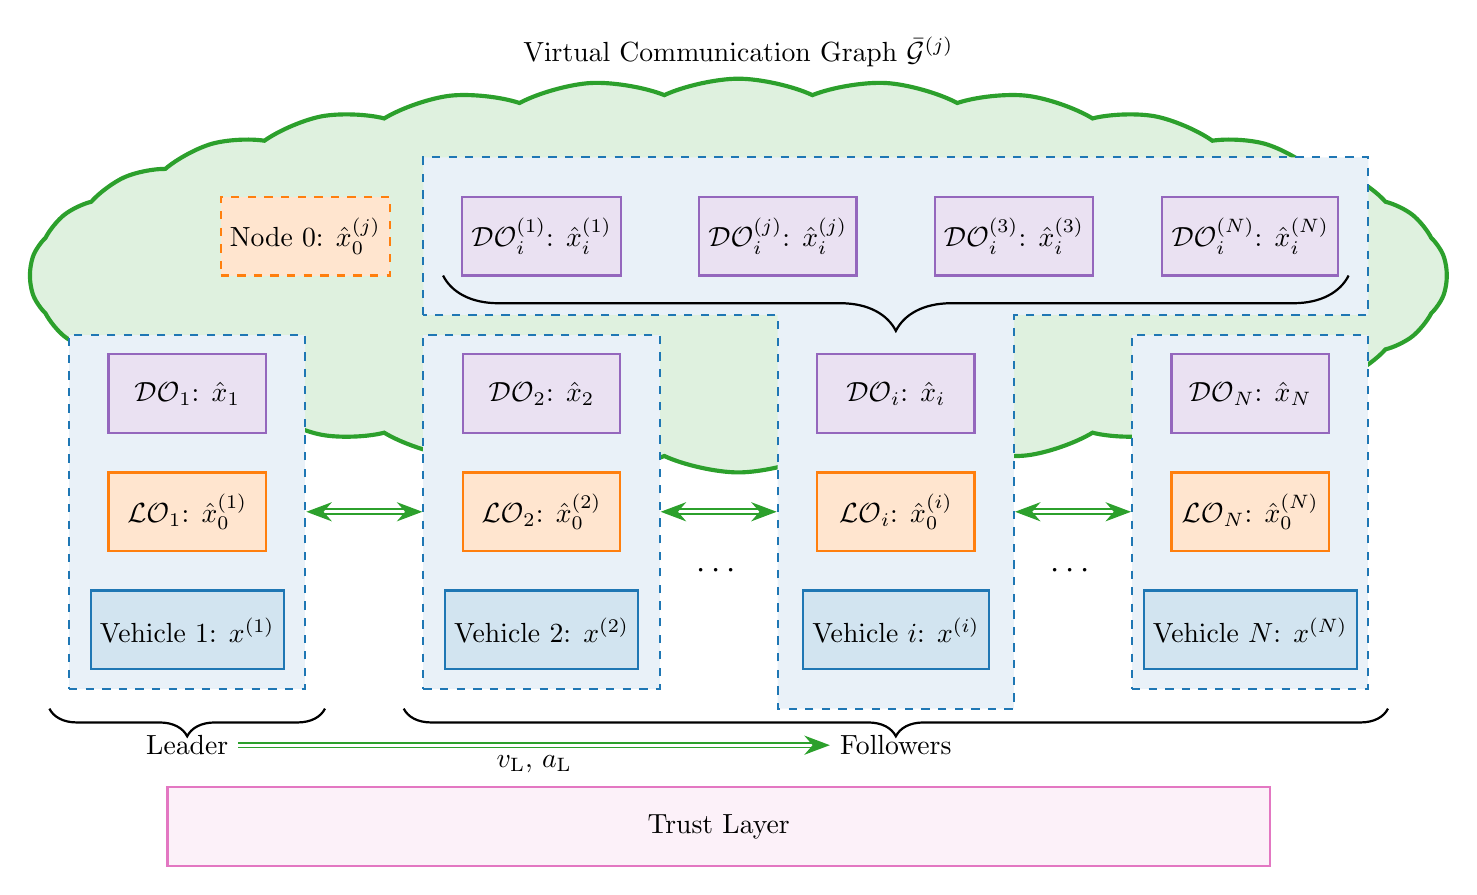
\begin{tikzpicture}[
    vehicle/.style={draw=blue1, fill=blue1!20, thick, minimum width=2cm, minimum height=1cm},
    localobs/.style={draw=orange1, fill=orange1!20, thick, minimum width=2cm, minimum height=1cm},
    distobs/.style={draw=purple1, fill=purple1!20, thick, minimum width=2cm, minimum height=1cm},
    sigarrow/.style={-stealth, thick, color=blue1},
    commarrow/.style={
    double,
    double distance=1pt,
    line width=0.7pt,
    draw=green1,
    {Stealth[scale=1.2]}-{Stealth[scale=1.2]}
    },
    physics/.style={draw=blue1, shape=rectangle, fill=blue1!10,line width=0.75pt,dashed,minimum width=3cm, minimum height=4.5cm}, %
    trust/.style={draw=rose1, shape=rectangle, fill=rose1!10,thick,minimum width=14cm, minimum height=1cm}
]
  %       		\draw [help lines,step=0.5cm] (0,0) grid (18,10); % 辅助网格 
		% % 画x和y轴坐标
		% \draw[stealth-,line width=2pt] (0,0)--(15,0);
		% % 画刻度
		% \foreach \x in {0,1,...,5}
		% {
		% 	\draw[xshift=\x cm] (0,0) -- (0,0.5);
		% };  
		% % 标坐标原点
		% \node[below] at (0,0){0};
		% %标x轴刻度值
		% \foreach \y in {1,2,...,18}
		% \node[below] at(\y,0){\y};

    \node[cloud,
            draw =green1,
            line width=1.5pt,
            text=cyan,
            cloud puffs = 30,
            cloud puff arc = 50,
            fill = green1!15,
            minimum width = 18cm,
            minimum height = 5cm,
            label=above:{Virtual Communication Graph $\bar{\G}^{(j)}$}
        ] (c) at(8.5, 4.5) {};
    
    \draw[draw=blue1,fill=blue1!10,dashed,line width=0.75pt] (4.5,4) -- (4.5,6)--(16.5,6) -- (16.5,4) -- (12,4) -- (12,-1) -- (9,-1) -- (9,4) -- (4.5,4) ;
    \draw [decorate, decoration={brace, mirror, amplitude=20pt}, thick]
    (4.75,4.5) -- (16.25,4.5);
    \draw [decorate, decoration={brace, mirror, amplitude=10pt}, thick]
    (4.25,-1) -- (16.75,-1)
    node[midway, below=6pt, name=followers] {Followers};
    \draw [decorate, decoration={brace, mirror, amplitude=10pt}, thick]
    (-0.25,-1) -- (3.25,-1)
    node[midway, below=6pt, name=leader] {Leader};
              
    \foreach \n in {1,2,3,4}
		{    
            \ifnum\n=3
                \node [name=PV\n,line width=0.75pt,minimum width=3cm, minimum height=4.5cm] at (4.5*\n-3,1.5) {};
            \else
                \node [physics,line width=0.75pt,name=PV\n] at (4.5*\n-3,1.5) {};
            \fi
            
            \ifnum\n=3
                \node[vehicle, name=V\n] at (4.5*\n-3, 0) {Vehicle $i$: $x^{(i)}$}; 
                \node[localobs,name=LO\n] at(4.5*\n-3,1.5) {$\LO_i$: $\hat{x}_{0}^{(i)}$};
                \node[distobs,name=DO\n] at(4.5*\n-3,3) {$\DO_i$: $\hat{x}_{i}$};
            \else
                \ifnum\n=4
                    \node[vehicle, name=V\n] at (4.5*\n-3, 0) {Vehicle $N$: $x^{(N)}$};
                    \node[localobs,name=LO\n] at(4.5*\n-3,1.5) {$\LO_N$: $\hat{x}_{0}^{(N)}$};
                    \node[distobs,name=DO\n] at(4.5*\n-3,3) {$\DO_N$: $\hat{x}_{N}$};
                \else
                    \node[vehicle, name=V\n] at (4.5*\n-3, 0) {Vehicle \n: $x^{(\n)}$}; 
                    \node[localobs,name=LO\n] at(4.5*\n-3,1.5) {$\LO_{\n}$: $\hat{x}_{0}^{(\n)}$};
                    \node[distobs,name=DO\n] at(4.5*\n-3,3) {$\DO_{\n}$: $\hat{x}_{\n}$};
                \fi
            \fi       
		};
    \foreach \j in {1,2,3,4}
    {
        \ifnum\j=2
                \node[distobs,name=DOi\j] at(3*\j+3,5) {$\DO_{i}^{(j)}$: $\hat{x}_{i}^{(j)}$};
            \else
                \ifnum\j=4
                    \node[distobs,name=DOi\j] at(3*\j+3,5) {$\DO_{i}^{(N)}$: $\hat{x}_{i}^{(N)}$};
                \else
                    \node[distobs,name=DOi\j] at(3*\j+3,5) {$\DO_{i}^{(\j)}$: $\hat{x}_{i}^{(\j)}$};
                \fi
            \fi
    
    };

    \node[localobs,name=node0,dashed] at(3,5) {Node 0: $\hat{x}_{0}^{(j)}$};
    \node[] at(8.25,0.75) {\large$\cdots$};
    \node[] at(12.75,0.75) {\large$\cdots$};

    \draw[commarrow,-{Stealth[scale=1.2]}] (leader) -- (followers) node[midway, below] {$v_{\text{L}}$, $a_{\text{L}}$};
    
    \draw[commarrow] (PV1) -- (PV2);
    \draw[commarrow] (PV2) -- (PV3);
    \draw[commarrow] (PV3) -- (PV4);

    \node[trust] at(8.25,-2.5) {Trust Layer};
    
    \end{tikzpicture}
    \caption{Schematic diagram of the estimation method.}
\end{figure*}

\begin{figure*}[h!]

    \centering
    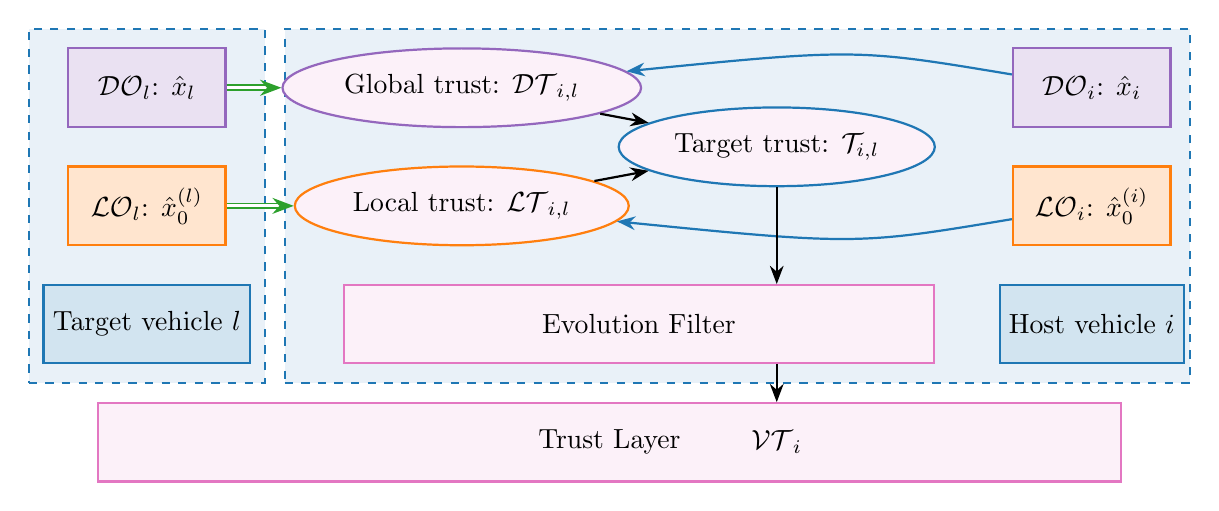
\begin{tikzpicture}[
    vehicle/.style={draw=blue1, fill=blue1!20, thick, minimum width=2cm, minimum height=1cm},
    localobs/.style={draw=orange1, fill=orange1!20, thick, minimum width=2cm, minimum height=1cm},
    distobs/.style={draw=purple1, fill=purple1!20, thick, minimum width=2cm, minimum height=1cm},
    sigarrow/.style={-Stealth, thick, color=blue1},
    commarrow/.style={
    double,
    double distance=1pt,
    line width=0.7pt,
    draw=green1,
    -Stealth
    },
    physics/.style={draw=blue1, shape=rectangle, fill=blue1!10,line width=0.75pt,dashed,minimum width=3cm, minimum height=4.5cm}, %
    trustlayer/.style={draw=rose1, shape=rectangle, fill=rose1!10,thick,minimum width=13cm, minimum height=1cm},
    trust/.style={draw=rose1, shape=ellipse, fill=rose1!10,thick,minimum width=1.5cm, minimum height=1cm}
]

  %     		\draw [help lines,step=0.5cm] (0,0) grid (18,10); % 辅助网格 
		% % 画x和y轴坐标
		% \draw[stealth-,line width=2pt] (0,0)--(15,0);
		% % 画刻度
		% \foreach \x in {0,1,...,5}
		% {
		% 	\draw[xshift=\x cm] (0,0) -- (0,0.5);
		% };  
		% % 标坐标原点
		% \node[below] at (0,0){0};
		% %标x轴刻度值
		% \foreach \y in {1,2,...,18}
		% \node[below] at(\y,0){\y};

        \node[physics,line width=0.75pt,minimum width=3cm, minimum height=4.5cm] at(2,1.5) { };
        \node[vehicle, name=target] at(2,0) {Target vehicle $l$};
        \node[localobs, name=LOt] at(2,1.5) {$\LO_{l}$: $\hat{x}_{0}^{(l)}$};
        \node[distobs, name=DOt] at(2,3) {$\DO_{l}$: $\hat{x}_{l}$};

        \node[physics,line width=0.75pt,minimum width=11.5cm, minimum height=4.5cm,name=host] at(9.5,1.5) {};
        \node[vehicle,name=host] at(14,0) {Host vehicle $i$};
        \node[localobs,name=LOh] at(14,1.5) {$\LO_{i}$: $\hat{x}_{0}^{(i)}$};
        \node[distobs,name=DOh] at(14,3) {$\DO_{i}$: $\hat{x}_{i}$};
        

        \node[trust,draw = purple1, name=DT] at(6,3) {Global trust: $\DT_{i,l}$};
        \node[trust,draw = orange1, name=LT] at(6,1.5) {Local trust:  $\LT_{i,l}$};
        \node[trust,draw = blue1, name=T] at(10,2.25) {Target trust: $\T_{i,l}$};
        % \node[trust] at(10,0) {$\VT_{i}$};

        \node[trust,shape=rectangle,name=evo, minimum width=7.5cm] at(8.25,0) {Evolution Filter}; 
        \node[name=evo,minimum height=1cm] at(10,0) {};

        \node[trustlayer] at(0.5/2+15.25/2,-1.5) {Trust Layer};
        \node[name = VT,minimum height=1cm] at(10,-1.5) {$\VT_{i}$};
    
        \draw[commarrow] (DOt) -- (DT);
        \draw[commarrow] (LOt) -- (LT);

        \draw[sigarrow] (LOh) .. controls +(-3,-0.5).. (LT);
        \draw[sigarrow] (DOh) .. controls +(-3,0.5).. (DT);

        \draw[sigarrow, black] (LT) -- (T);
        \draw[sigarrow,black] (DT) -- (T);

        \draw[sigarrow,black] (T) -- (evo);
        \draw[sigarrow,black] (evo) -- (VT);

        
        
    \end{tikzpicture}
    \caption{Trust framework.}
    \label{fig_trust_framwork}

\end{figure*}







\bibliographystyle{IEEEtran}


%=================
\bibliography{biblio}
%=================
\end{document}